\documentclass[12pt,a4paper,english]{book}
\usepackage{babel}
\usepackage{ae}
\usepackage{aeguill}
\usepackage{shortvrb}
\usepackage[latin1]{inputenc}
\usepackage{tabularx}
\usepackage{longtable}
\setlength{\extrarowheight}{2pt}
\usepackage{amsmath}
\usepackage{graphicx}
\usepackage{color}
\usepackage{multirow}
\usepackage{ifthen}
\usepackage[DIV12]{typearea}
% generated by Docutils <http://docutils.sourceforge.net/>
\newlength{\admonitionwidth}
\setlength{\admonitionwidth}{0.9\textwidth}
\newlength{\docinfowidth}
\setlength{\docinfowidth}{0.9\textwidth}
\newlength{\locallinewidth}
\newcommand{\optionlistlabel}[1]{\bf #1 \hfill}
\newenvironment{optionlist}[1]
{\begin{list}{}
  {\setlength{\labelwidth}{#1}
   \setlength{\rightmargin}{1cm}
   \setlength{\leftmargin}{\rightmargin}
   \addtolength{\leftmargin}{\labelwidth}
   \addtolength{\leftmargin}{\labelsep}
   \renewcommand{\makelabel}{\optionlistlabel}}
}{\end{list}}
\newlength{\lineblockindentation}
\setlength{\lineblockindentation}{2.5em}
\newenvironment{lineblock}[1]
{\begin{list}{}
  {\setlength{\partopsep}{\parskip}
   \addtolength{\partopsep}{\baselineskip}
   \topsep0pt\itemsep0.15\baselineskip\parsep0pt
   \leftmargin#1}
 \raggedright}
{\end{list}}
% begin: floats for footnotes tweaking.
\setlength{\floatsep}{0.5em}
\setlength{\textfloatsep}{\fill}
\addtolength{\textfloatsep}{3em}
\renewcommand{\textfraction}{0.5}
\renewcommand{\topfraction}{0.5}
\renewcommand{\bottomfraction}{0.5}
\setcounter{totalnumber}{50}
\setcounter{topnumber}{50}
\setcounter{bottomnumber}{50}
% end floats for footnotes
% some commands, that could be overwritten in the style file.
\newcommand{\rubric}[1]{\subsection*{~\hfill {\it #1} \hfill ~}}
\newcommand{\titlereference}[1]{\textsl{#1}}
% end of "some commands"
% de-uglify paragraphs
\setlength{\parindent}{0pt}
\setlength{\parskip}{\medskipamount}

% prettify fonts
\usepackage[T1]{fontenc}
\usepackage{cmbright}
\ifthenelse{\isundefined{\hypersetup}}{
\usepackage[colorlinks=true,linkcolor=blue,urlcolor=blue]{hyperref}
}{}
\title{Application development with Edje}
\author{}
\date{}
\hypersetup{
pdftitle={Application development with Edje},
pdfauthor={Andres Blanc}
}
\raggedbottom
\begin{document}
\maketitle
%___________________________________________________________________________
\begin{center}
\begin{tabularx}{\docinfowidth}{lX}
\textbf{Title}: &
	Application development with Edje \\
\textbf{Subtitle}: &
	From the very basics \\
\textbf{Author}: &
	Andres Blanc \\
\textbf{Contact}: &
	\href{mailto:andresblanc@gmail.com}{andresblanc@gmail.com} \\
\textbf{Version}: &
	1.0 \\
\textbf{Date}: &
	2008/04/03 \\
\textbf{Copyright}: &
	This book is distributed under the terms of the Attribution-ShareAlike
CC license. See: \href{http://creativecommons.org/licenses/by-sa/3.0/}{http://creativecommons.org/licenses/by-sa/3.0/}. \\
\end{tabularx}
\end{center}

\setlength{\locallinewidth}{\linewidth}


\subsubsection*{~\hfill Abstract\hfill ~}

An introduction to GUI based application development. Starts from
the most basic concepts and introduces the EFL libraries that deal
with each of them. It covers Edje, Ecore, Evas and EWL. This book
is intended to cover all the concepts needed by a novice programmer
to create a full blown Edje based application.

\hypertarget{contents}{}
\renewcommand{\contentsname}{Contents}
\tableofcontents

\bigskip
\label{contents}


%___________________________________________________________________________

\hypertarget{book-overview}{}
\chapter{Book overview}
\label{book-overview}

I. \href{\#about-graphical-user-interfaces}{About Graphical User Interfaces}.
If we look through the code of some of the many open source applications
available, we can find most of them share a common structure. This chapter
introduces the reader to said structure, to the concept of an Event loop and
how does it deal with the interaction between form and function.

I.I. \href{\#decomposing-the-frontend}{Decomposing the frontend}.
There are different approaches to the creation of Graphical User Interfaces,
some provide flexibility while others shorter development time. In the end, the
rest of the application will have to go through the same mechanism to deal
with the interface.

I.II. \href{\#introduction-to-edje}{Introduction to Edje}.
Edje is a compromise between flexibility and development time. Comparing it to
a plain canvas or a fully featured toolkit can show us how it fits in the
middle ground and provides advantages for designers and developers alike.

I.III. \href{\#the-foundations}{The foundations}.
Edje allows low level control of the interface without forcing the developer
through a low level API. The interface objects are implemented as Evas objects,
but through a completely new language friendly to designers and independent
from the application code.

I.IV. \href{\#convenient-libraries}{Convenient libraries}
To load an Edje interface the application needs to setup an Evas canvas first.
This would look as a burden for the developer, dealing with issues specific to
the underlying system. Thankfully Evas is supported by an additional library
that resolve most of these issues, Ecore.

II. \href{\#the-foundations-in-practice}{The foundations in practice}.
Practical examples of the Englighenment Foundation Libraries required for a
common Edje application.

II.I. \href{\#working-with-the-canvas}{Working with the canvas}.
Including new Edje objects inside the previously setup canvas can be explained
with this simple example.

II.II. \href{\#interacting-with-the-objects}{Interacting with the objects}.
There are different channels for the application to interact with the
interface. For the sake of brevity I will include an example of each one to
serve as an introduction for the practical examples to come in the next
chapters.

II.III. \href{\#building-a-framework}{Building a framework}.
- An brief introduction to the concept of the framework
- Code sample of the main.c file and general explanation

II.III.I. \href{\#getting-the-interface-up}{Getting the interface up}.
- A mention of the environment{\_}init/shutdown functions without code examples
- A code sample + explanation of the the window creation functions

II.III.II. \href{\#settings-are-important-too}{Settings are important too}.
- An brief introduction to Ecore{\_}Config (refer to the cookbook).
- A code sample + explanation of functions that deal with multiple theme files.

II.III.III. \href{\#simpler-interface-management}{Simpler interface management}.
- A code sample + explanation of the functions that fetch the theme objects

III. \href{\#introduction-to-widgets}{Introduction to widgets}.
Interfaces need to resolve two problems, presenting information to users and
taking orders from them. The past chapters presented enough information to
solve the first. In the following chapters we will review the second.

III.I. \href{\#widgets-with-edje}{Widgets with Edje}.
Since this is a book about Edje it might be a good idea to detail the way Edje
simplifies custom widget creation by reviewing the list of tasks presented in
the previous chapter and how Edje helps with each task.


%___________________________________________________________________________

\hypertarget{about-graphical-user-interfaces}{}
\chapter{About Graphical User Interfaces}
\label{about-graphical-user-interfaces}

So... you want to create a GUI application? I assume so since you choosed this
book as instructive, or at least bathroom, material. You could google ``GUI'' and
``library'' to feel overwhelmed by the large number of development libraries
avilable. As you look through the source of your (open source) favorites you
will realize that all of them, and the applications that use them, share a
common structure. In this chapter we will review that structure.

At this point it is convenient to note that the concepts seen in this book and
the applications resulting from them translate painlessly to special purpose
computers or embed devices running under alternative architectures like ARM or
PPC. Edje and related libraries are not only efficient but portable.

The structure of the averange graphical application is built around a concept
known as event (or signal) driven execution. Event driven applications are
persistent and depend on a gate guardian to call the appropriate functions in
the appropriate moment. This gate guardian is known as the Event loop (or main
loop).

{\hfill\includegraphics[width=0.850\linewidth]{img/graphical_application_components.png}\hfill}

The functions that form a event driven application (with a GUI) can be split
among two groups. The first group is know as the backend, these functions deal
with the actual purpose of the application, crunching numbers, decoding media
files and so on. The second group is known as the frontend, the prupose of
these functions is to present the results from the backend to their human
overlords and to receive orders from them.

Between the backend and the frontend is where the Event loop lives, its mission
is to connect both ends of the application. Not only between them but also with
their environment. The Event loop mantains a list of signals to look out for
and functions related to them. When a signal is received, the Event loop look
it up in a list and executes the corresponding function or functions.

For the application to work, the Event loop needs to be aware of events in the
interface, thus it is  usually provided by the same library that provides the
GUI elements. It also needs to be aware of events in the system where the
application is running. Even when the concept is simple, creating a portable
and properly abstracted event loop is no simple task.


%___________________________________________________________________________

\hypertarget{decomposing-the-frontend}{}
\section{Decomposing the frontend}
\label{decomposing-the-frontend}

There are many libraries that aid creation of a GUI. From a plain canvas
consisting of primitive design objects, like a line or a rectangle, to complex
layout schemes and predefined interface elements, the latter known as ``toolkit''
or widget library. As opposed to the first, in a toolkit the canvas is just
another widget.

Regardless of the method of choice, the resulting GUI has to provide the same
resources to the rest of the application. A mechanism to present information
to the user, a mechanism to know when the user interacts with the interface and
a mechanism to retreive information that resulted from said interaction.

In the case of the plain canvas the application developer must assemble the
interface elements, know as widgets, using primitive objects. A very simple
text entry widget could consist of a rectangle and a string of text. Besides
assembling the widget, the developer has to instruct the Event loop  to call a
given function on a given interface event on either primitive object. It is
possible to discriminate between, for example, a click in the rectangle from a
click in the string.

In the case of a toolkit library the application developer would simply include
a predefined ``text entry'' widget. The events from this object would be dealt
with in terms of the object as a whole. It wouldn't seem that there is much
difference between using a canvas or using a toolkit library until we consider
all the possiblities, like focus, overflowing text, copying, pasting,
selecting, etc.

Deciding which approach to use is, of course, up to the developer to decide as
each one provide capabilities useful for different types of applications. But
as we will find out further ahead in this book, these examples only represent
opposite extremes and there is an alternative approach that sits quite
comfortably in the middle. Edje.


%___________________________________________________________________________

\hypertarget{introduction-to-edje}{}
\section{Introduction to Edje}
\label{introduction-to-edje}

Allow me to begin this chapter with a quote from the introduction of Edje's API
Reference. After all, I cannot expect to give Edje a better introduction than
its creator:
\begin{quote}

Edje is a complex graphical design and layout library. {[}..{]}

{[}..{]} Edje should serve all the purposes of creating visual elements
(borders of windows, scrollbars, etc.) and allow the designer the ability
to animate, layout and control the look and feel of any program using Edje
as its basic GUI constructor. This library allows for multiple collections
of Layouts in one file, sharing the same image database and thus allowing a
whole theme to be conveniently packaged into 1 file and shipped around.

Edje {[}..{]} separates the layout and behavior logic. Edje files ship with an
image database, used by all the parts in all the collections to source
graphical data. {[}..{]} Each part collection consists of a list of visual
parts, as well as a list of programs. A program is a conditionally run
program that if a particular event occurs (a button is pressed, a mouse
enters or leaves a part) will trigger an action that may affect other
parts. In this way a part collection can be ``programmed'' via its file as to
hilight buttons when the mouse passes over them or show hidden parts when a
button is clicked somewhere etc. The actions performed in changing from one
state to another are also allowed to transition over a period of time,
allowing animation.

{[}..{]} This separation and simplistic event driven style of programming can
produce almost any look and feel one could want for basic visual elements.
Anything more complex is likely the domain of an application or widget set
that may use Edje as a convenient way of being able to configure parts of
the display.
\end{quote}

As we have seen in the past chapters, there are roughly two methods for
creating Graphical User Interfaces. In both cases it had to be implemented
through a programming language. In one case, an API was used by the application
developer to assemble interface elements from more primitive objects, in the
other case the API was used to include objects already defined by a library.
Any changes to an nterface object beyond simplistic style modifications had to
be submitted by the designer to the developer. Layout changes were only
slightly less difficult than behavior changes. The idea of working on the
interface objects and their composition in a live environment, like a web
developer does, was pretty much unthinkable.

This is where the Edje library fits in, it liberates the designer and the
developer from eachother. The artists uses the Edje Data Collection language to
manipulate primitive objects. EDC is in some ways comparable to Cascading Style
Sheets but its free of the framework that markup imposes. From the other side,
the developer only has to include the resulting object and setup the callbacks
(by the main loop) to the backend functions.

{\hfill\includegraphics[width=0.850\linewidth]{img/workflow.png}\hfill}

Except for the usage of nested blocks, the sintax of an EDC file is similar to
CSS. What really sets them appart is that with EDC the designer it's free to
create and layout design elements as he sees fit. With CSS the designer is
limited to applying style and layout properties to a structure of objects
defined by the markup. With Edje each design object, know as ``part'', is created
by the designer and the final interface object composed by those parts, known
as ``group'', is used by the developer. The resulting theme file can consist of
multiple groups representing multiple interface object.

The application developer will find out that the Edje API is small, since the
developer is not expected to alter the composition of a group. The API focus on
high level manipulation of groups, like forcing a maximum size, but provides
some functions to alter the content of a part when it's necessary to transmit
information, like altering a paragraph of text with a message.

If we compare Edje to both extremes of GUI development we can see it provides
the flexibility of developing your own interface objects from a plain canvas,
yet remain almost as simple as including a predefined object from a toolkit. Of
course Edje has shortcomings of its own and we will explore them in this book
as well.


%___________________________________________________________________________

\hypertarget{the-foundations}{}
\section{The foundations}
\label{the-foundations}

From a developer's point of view, we cannot expect to understand how Edje works
without going through a brief introduction about the Evas first. Luckily for
this writer, an excellent introduction to Evas has already been written in the
API Reference.
\begin{quote}

Evas is a clean display canvas API for several target display systems that
can draw anti-aliased text, smooth super and sub-sampled scaled images,
alpha-blend objects much and more.

It abstracts any need to know much about what the characteristics of your
display system are or what graphics calls are used to draw them and how. It
deals on an object level where all you do is create and manipulate objects
in a canvas, set their properties, and the rest is done for you.

Evas optimises the rendering pipeline to minimise effort in redrawing
changes made to the canvas and so takes this work out of the programmers
hand, saving a lot of time and energy.

It's small and lean, designed to work on embedded systems all the way to
large and powerful multi-cpu workstations. It can be compiled to only have
the features you need for your target platform if you so wish, thus keeping
it small and lean. It has several display back-ends, letting it display on
several display systems, making it portable for cross-device and
cross-platform development.
\end{quote}

When using the Evas API directly, the developer uses function calls n the format
object{\_}line{\_}add and object{\_}image{\_}add to include the different primitives in our
canvas. Each of these primitives would be included in the form of an ``Evas
object''.

But Evas is not limited to simply rendering primitive objects. The most common
use for a canvas is to assemble multiple primitives like lines or rectangles
into figures like charts or diagrams. In order to maintain coherency among all
the primitives the developer was forced to implement functions that abstracted
manipulation of the figure from the manipulation of its components. One of
these ``workarounds'' is now known as Evas Smart Objects.

Smart objects are implemented by the developer to create new Evas object types.
Functions like add, del, hide, show are implemented using the regular Evas API
to affect each primitive. This collection of functions is grouped into a new
Evas Smart Class structure that consist of a list of pointers to the functions,
the object type name and version. The instances resulting from these classes
would be manipulated by the canvas in the same way it does for any other
object.

Edje is implemented as a more abstract type of smart object. The list of
primitives to manipulate is not hard coded into the functions forming the Smart
Class. Edje has functions that analyze the structure of a compiled theme file
and get the list of primitives and their properties from a given ``group'' inside
the file.

In the end Edje interfaces can be seen as an illustration over a canvas. Space
they can share with other primitive and smart objects. Without an Evas canvas
there is no Edje theme.


%___________________________________________________________________________

\hypertarget{convenient-libraries}{}
\section{Convenient libraries}
\label{convenient-libraries}

The normal process to get a canvas up and running can be bothersome. Evas
supports multiple rendering engines, like the software, xrender and opengl
flavors of X11 and framebuffer devices. But before any rendering can be done
the developer has to complete an Evas{\_}Engine{\_}Info structure with the required
information about the target engine. This forces the developer to research the
different functions to get that information for each target. Alternatively he
can use a shortcut available for most of them.

As you might have realized by at this point, I intend to quote the official API
reference at every chance I get. This one comes straight from the ``The Ecore
Main Loop'' page:
\begin{quote}

Ecore is a clean and tiny event loop library with many modules to do lots
of convenient things for a programmer, to save time and effort.

It's small and lean, designed to work on embedded systems all the way to
large and powerful multi-cpu workstations. It serializes all system
signals, events etc. into a single event queue, that is easily processed
without needing to worry about concurrency. A properly written,
event-driven program using this kind of programming doesn't need threads,
nor has to worry about concurrency. It turns a program into a state
machine, and makes it very robust and easy to follow.
\end{quote}

At the beginning of its life, the Ecore library was used as a Event loop and
loop management is still one of the modules that composes Ecore.

{\hfill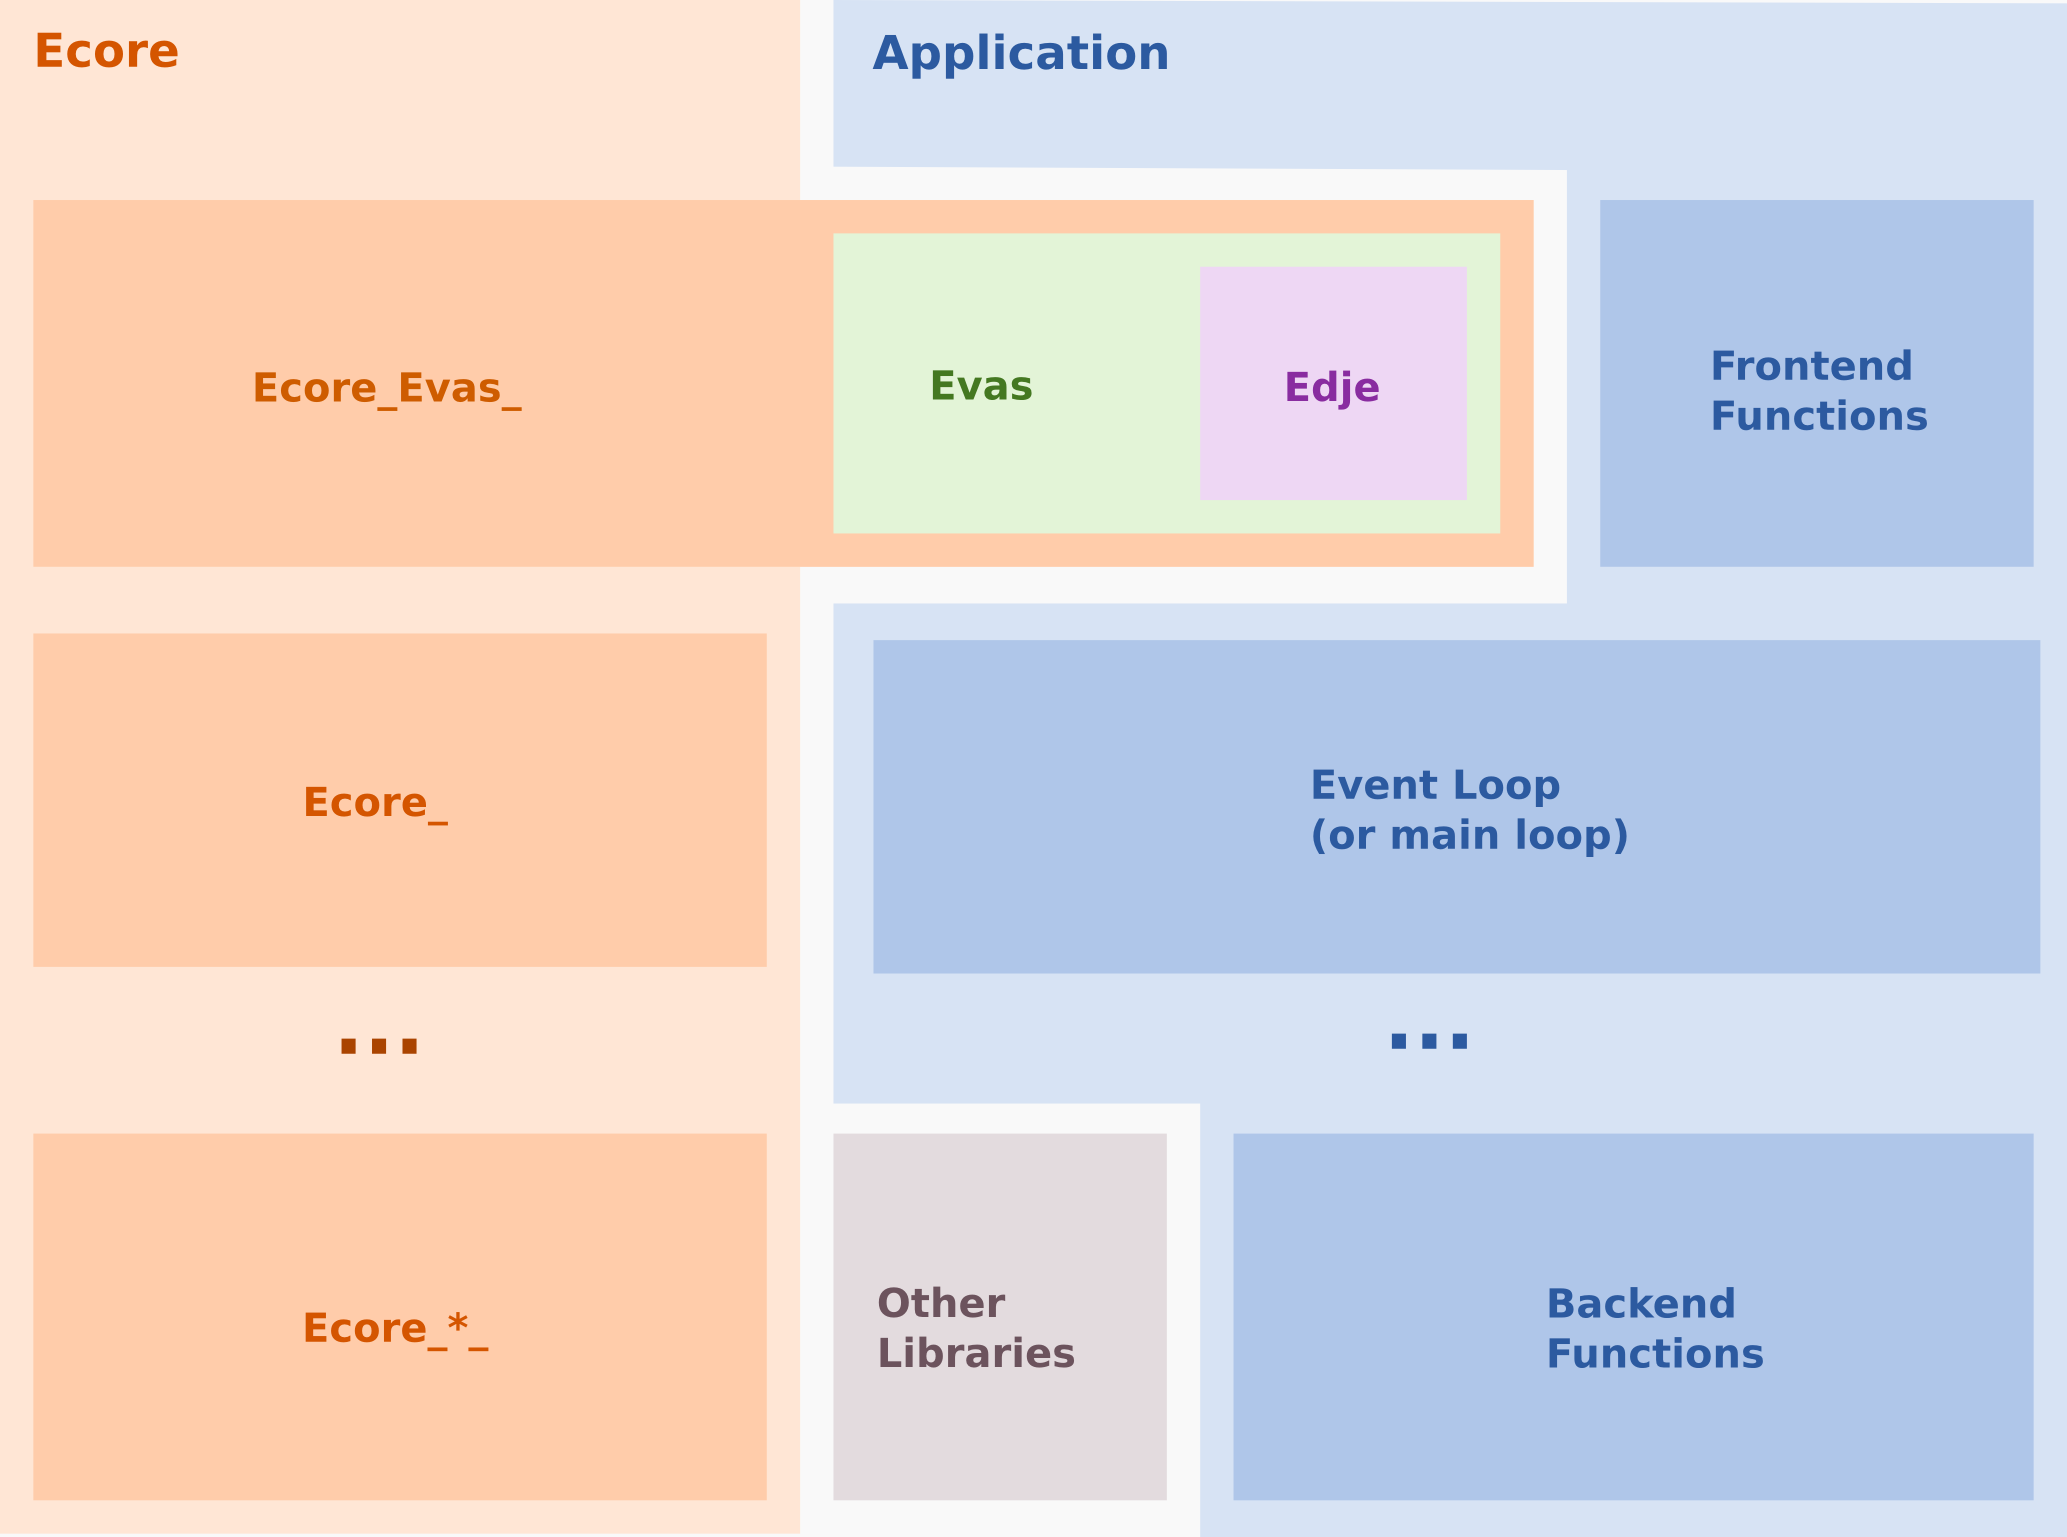
\includegraphics[width=0.850\linewidth]{img/required_libraries.png}\hfill}

Today, Ecore encompasses a long list of modules properly namespaced and
prefixed with ``Ecore{\_}''. From what we have seen in the previous chapters, there
are two modules that jump right out of the list. The first Ecore{\_}Evas and
second named Ecore. The first provides convenient functions to setup the Evas
canvas and the later provides the loop management functionality described
above.

The developer needs an Evas canvas to render the Edje interface and Ecore{\_}Evas
is the simplest way to get an Evas canvas up and running. This wrapper is
intended to support every backend that Evas supports with its respective (and
sometimes unique) attributes. It trivializes initialization to a couple of
lines and multiple engine support to an application reload.


%___________________________________________________________________________

\hypertarget{the-foundations-in-practice}{}
\chapter{The foundations in practice}
\label{the-foundations-in-practice}

By pointing out that the Enlightenment Foundation Libraries are designed in a
Object Oriented manner I wish not to raise the wrath of OO purists but to
simplify the mental image of the structure of the EFL C API in the reader's
imagination.

Now that the pitchforks are back in the barn allow me to put it in more clear
terms with a simple example:
\begin{quote}{\ttfamily \raggedright \noindent
Evas{\_}Object~*button~=~NULL;~\\
button~=~edje{\_}object{\_}add(evascanvas);~\\
edje{\_}object{\_}file{\_}set(button,~"theme.edj",~"button");
}\end{quote}

This is a simple C snippet that could be translated into a more (sintactically
speaking) object oriented language like Python as:
\begin{quote}{\ttfamily \raggedright \noindent
button~=~Evas{\_}Object()~\\
button.file{\_}set("theme.edj","button")
}\end{quote}

The differences between the code snippets could be written off as ``sintactic
sugar'' but it serves to demonstrate the structure which the EFL C API follows.
If we dissected the last function call we could split it into three groups.
First, the class of the object to manipulate, \texttt{edje{\_}object}, second, the
method to call \texttt{file{\_}set} and third the pointer to the object instance
\texttt{(button,} along with the parameters \texttt{"theme.edj","button")} or, in more
generic terms, \texttt{class{\_}method(instance,parameters)}.

The first source snippet in the following tutorial is, of course, the first
exception. The following function calls deal with the library itself. Anyway,
displaying a simple Edje object in a window is a task with a few well defined
steps that begin by initializing the necessary libraries:
\begin{quote}{\ttfamily \raggedright \noindent
{\#}include~<stdlib.h>~\\
{\#}include~<stdio.h>~\\
{\#}include~<Evas.h>~\\
{\#}include~<Ecore.h>~\\
{\#}include~<Ecore{\_}Evas.h>~\\
~\\
int~main()~{\{}~\\
~~~~if~(!ecore{\_}init())~return~EXIT{\_}FAILURE;~\\
~~~~if~(!ecore{\_}evas{\_}init())~return~EXIT{\_}FAILURE;~\\
~~~~...
}\end{quote}

All initialize-able Enlightenment Foundation Libraries do so in the format
\texttt{library{\_}name{\_}init()}. Both Ecore and Ecore{\_}Evas need to be initialized
before being used and both will return success or failure using standard C
values (0 is failure, any other number is success), hence the \texttt{if}.

This would be a good moment to note that the assembled, and commented, version
of the source code of these examples can be found in CVS repository of the
Enlightenment project: \texttt{docs/devwithedje/src}

In order to render a canvas its necessary to create a canvas wrapper that will
host it and to store a pointer to it for future reference:
\begin{quote}{\ttfamily \raggedright \noindent
...~\\
Ecore{\_}Evas~~*ecore{\_}evas~=~NULL;~\\
...~\\
ecore{\_}evas~=~ecore{\_}evas{\_}software{\_}x11{\_}new(NULL,~0,~0,~0,~800,~600);~\\
if~(!ecore{\_}evas)~return~EXIT{\_}FAILURE;~\\
...
}\end{quote}

While the software{\_}x11 engine is being used in this example, its possible to
use any other supported engine by simply changing the second line to
\texttt{ecore{\_}evas{\_}enginename{\_}new()}. A list of supported engines and their
parameters can be found in the Official API reference.

Once the canvas wrapper has been setup we need to change its state to visible:
\begin{quote}{\ttfamily \raggedright \noindent
...~\\
ecore{\_}evas{\_}title{\_}set(ecore{\_}evas,~"Example~Application");~\\
ecore{\_}evas{\_}name{\_}class{\_}set(ecore{\_}evas,~"testapp",~"Testapp");~\\
ecore{\_}evas{\_}show(ecore{\_}evas);~\\
...
}\end{quote}

While the first two lines are optional, it is useful to see the way we set the
title name and class of the window that will host our canvas. The third
function sets the given canvas wrapper to visible, this can be reversed later
with \texttt{ecore{\_}evas{\_}hide()}.

The canvas wrapper is ready to go, but the actual canvas that will be use to
draw our Edje objects is nowhere to be found:
\begin{quote}{\ttfamily \raggedright \noindent
...~\\
Evas~*evas~=~NULL;~\\
...~\\
evas~=~ecore{\_}evas{\_}get(ecore{\_}evas);~\\
...
}\end{quote}

The function ecore{\_}evas{\_}get() returns a pointer to the canvas housed in the
canvas wrapper, this is the pointer we need in order to include our Edje
objects later.

The execution loop for the program can also be conveniently handled by Ecore:
\begin{quote}{\ttfamily \raggedright \noindent
...~\\
ecore{\_}main{\_}loop{\_}begin();~\\
...
}\end{quote}

Once ecore{\_}main{\_}loop{\_}begin(..) has been called, both the canvas wrapper and
the canvas itself will be drawn in their current state (a 800x600px empty
window in this case). Ecore will continue to loop until an event handled by it
occurs.

Once the execution of the main loop has finished it's a good practice to shut
down any library we initiated:
\begin{quote}{\ttfamily \raggedright \noindent
~~~~...~\\
~~~~ecore{\_}evas{\_}shutdown();~\\
~~~~ecore{\_}shutdown();~\\
{\}}~\\
...
}\end{quote}


%___________________________________________________________________________

\hypertarget{working-with-the-canvas}{}
\section{Working with the canvas}
\label{working-with-the-canvas}

Now that we know how to setup the enviroment to display the Edje objects we
will review how to include and interact with the objects themselves. The
following code is platform independent and can be merged with the example code
provided before or with the equivalent for any other platform.

Just like the last time we begin by including the necessary header files and
initializing the libraries:
\begin{quote}{\ttfamily \raggedright \noindent
...~\\
{\#}include~<Edje.h>~\\
...~\\
int~main()~{\{}~\\
~~~~...~\\
~~~~if~(!edje{\_}init())~return~EXIT{\_}FAILURE;~\\
~~~~...
}\end{quote}

After a pointer to the canvas has been aquired, we need a pointer to a valid
Evas object to insert our Edje object:
\begin{quote}{\ttfamily \raggedright \noindent
...~\\
Evas{\_}Object~*edje~=~NULL;~\\
...~\\
edje~=~edje{\_}object{\_}add(evas);~\\
edje{\_}object{\_}file{\_}set(edje,~"testfile.edj",~"testgroup");~\\
...
}\end{quote}

Both functions are specific to Edje, in the first case we use edje{\_}object{\_}add
to create a pointer to an Evas object and edje{\_}object{\_}file{\_}set to add the
contents represented by ``testgroup'' in ``testfile.edj''.

As with any other Evas object we need to instruct Evas to make it visible, but
not before adjusting the object inside the canvas or since we are only showing
one object, adjust the canvas to the size of our object:
\begin{quote}{\ttfamily \raggedright \noindent
...~\\
Evas{\_}Coord~width,~height;~\\
...~\\
evas{\_}object{\_}move(edje,~0,~0);~\\
edje{\_}object{\_}size{\_}min{\_}get(edje,~{\&}amp;width,~{\&}amp;height);~\\
evas{\_}object{\_}resize(edje,~width,~height);~\\
ecore{\_}evas{\_}resize(ecore{\_}evas,~width,~height);~\\
evas{\_}object{\_}show(edje);~\\
...
}\end{quote}

First we use evas{\_}object{\_}move to move our Edje object to the left-most, up-most
corner of the canvas. The function edje{\_}object{\_}size{\_}min{\_}get, returns the
minimal possible size of the object and evas{\_}object{\_}resize changes the current
size of the object to those values.

Before the end, we resize the canvas to the same values the object has with
ecore{\_}evas{\_}resize and (finally) instruct Evas to show the object.


%___________________________________________________________________________

\hypertarget{interacting-with-the-objects}{}
\section{Interacting with the objects}
\label{interacting-with-the-objects}

To understand how to interact with Edje or any other Evas based object we need
to review the basics of how the main loop manager handles events. Ecore
maintains a list of pointers to functions to be called when a signal of a given
type is received. These functions are known as signal ``handlers''.

By default, Ecore awareness is limited to system singals like HUP or KILL.
Additional libraries or modules like Ecore{\_}Evas register new signal types for
the event loop to be aware of. In the specific case of Evas the new signal
types deal with the interaction between the user and the Evas objects displayed
in the canvas.

The developer can manipulate the list of handlers as well as creating new
signal types. The latter among other subjects like timers and pollers exceed
the scope of this book and are properly documented by the API reference and the
EFL Cookbook.

We will begin by setting up a simple signal handler that will be called any
time the application is closed:
\begin{quote}{\ttfamily \raggedright \noindent
Ecore{\_}Event{\_}Handler*~close~=~NULL;~\\
...~\\
int~\\
good{\_}bye(void~*data,~int~type,~void~*event)~\\
{\{}~\\
~~~~//Removing~handler~for~no~reason~other~than~API~showoff~\\
~~~~if~(ecore{\_}event{\_}handler{\_}del(close))~\\
~~~~~~~~printf("Handler~deleted{\textbackslash}n");~\\
~\\
~~~~printf("Good~bye!~{\textbackslash}n");~\\
~~~~ecore{\_}main{\_}loop{\_}quit();~\\
~~~~ecore{\_}evas{\_}shutdown();~\\
~~~~ecore{\_}shutdown();~\\
~~~~edje{\_}shutdown();~\\
{\}}~\\
...~\\
int~main()~{\{}~\\
...~\\
~~~~close~=~ecore{\_}event{\_}handler{\_}add(ECORE{\_}EVENT{\_}SIGNAL{\_}EXIT,~\\
~~~~~~~~~~~~~~~~~~~~~~~~~~~~~~~~~~~~good{\_}bye,"data");~\\
~~~~...~\\
~~~~ecore{\_}main{\_}loop{\_}begin();~\\
~~~~...
}\end{quote}

This example moves the library shutdown procedure from the main function to the
``good{\_}bye'' function. Then before the main loop is initiated we add the handler
for this signal type. The last parameter it's a pointer to any kind of data you
want to pass to the handler function, in this case is just a string containing
``data''.

Interaction with the interface works in a similar way. The Edje library
registers its own handler function in the Ecore loop. This handler will be
called for every signal coming from the interface. Therefore, in order to react
to interface events we need to register our functions as ``callbacks'' in this
handler's list:
\begin{quote}{\ttfamily \raggedright \noindent
...~\\
void~\\
colorize(void~*data,~Evas{\_}Object~*o,~const~char~*emission,~\\
~~~~~~~~~const~char~*source)~\\
{\{}~\\
~~~~Evas{\_}Coord~x,y;~\\
~~~~evas{\_}pointer{\_}canvas{\_}xy{\_}get(evas,{\&}amp;x,{\&}amp;y);~\\
~~~~if(x~>~255)~x~=~255;~\\
~~~~if(y~>~255)~y~=~255;~~~~~~~~~~~~~//R,~~~G,~~~B,~~~A,~\\
~~~~edje{\_}color{\_}class{\_}set("main~color",~190,~x,~~~y,~~~255,~\\
~~~~~~~~~~~~~~~~~~~~~~~~~~~~~~~~~~~~~~~255,~255,~255,~255,~\\
~~~~~~~~~~~~~~~~~~~~~~~~~~~~~~~~~~~~~~~255,~255,~255,~255);~\\
{\}}~\\
...~\\
int~main()~{\{}~\\
~~~~...~\\
~~~~edje{\_}object{\_}signal{\_}callback{\_}add(edje,~"mouse,move",~"*",~\\
~~~~~~~~~~~~~~~~~~~~~~~~~~~~~~~~~~~~colorize,"data");~\\
~~~~...~\\
~~~~ecore{\_}main{\_}loop{\_}begin();~\\
~~~~...
}\end{quote}

The resulting application changes the color of every part using the ``main
color'' color class every time the mouse moves inside the interface. If you use
the EDC theme included in the assembled example the result will be a small
rectangle in the middle of the canvas that changes of color as we move our
mouse around.

The function that produces this effect is our handler, or callback, \texttt{colorize}.
We call functions from the Evas API \texttt{evas{\_}pointer{\_}canvas{\_}xy{\_}get} and the Edje
API \texttt{edje{\_}color{\_}class{\_}set}. The first call gets the current coordinates of
the mouse pointer position. The second call uses those values to alter the
color class ``main color''.

Before the main loop begins we use \texttt{edje{\_}object{\_}signal{\_}callback{\_}add} to
register our callback. The real handler keeps its own list of functions to call.
This list's index is a combination of the signal identification and the name of
the source that emitted it. In this particular case, the function \texttt{colorize}
will be called when the signal ``mouse,move'' is emitted by any object in the
interface. Edje string matching supports wildcards for both the name and source
of the signal.


%___________________________________________________________________________

\hypertarget{building-a-framework}{}
\section{Building a framework}
\label{building-a-framework}

Hopefully the reader has not been introduced to the concept of software
frameworks by web based monsters like Ruby on Rails. Personally I think RoR is
great, my point is that a framework does not necessarily mean big complex,
abstract software libraries. A framework can be seen as the standardization of
common, complex tasks into a library shared by group of applications. With a
framework short development times means a compromise with flexibility.

In this section and the following subsections we will develop an application
framework for applications with a specific profile. An X11 desktop application
that doesn't require any exotic manipulation of its theme files and with a
interface simple enough that all its objects can be laid out using a single
Edje object.

The tasks that this framework will take care of are pretty straight forward:
* Maintain a configuration file (in the default location used by Ecore{\_}Config).
* Setup the window properties and main layout from a theme object.
* Manage theme objects, including changing a theme file on runtime and
maintaining two the files, current and default.

The example application will be an Edje group viewer, this application will
receive a filename and a group name, it will display the application inside a
viewport, print the last signal emitted by the group and provide a minimap for
navigating the viewport. Without further ado, here it is, the main file:

Literal block expected; none found.



%___________________________________________________________________________

\hypertarget{getting-the-interface-up}{}
\subsection{Getting the interface up}
\label{getting-the-interface-up}


%___________________________________________________________________________

\hypertarget{settings-are-important-too}{}
\subsection{Settings are important too}
\label{settings-are-important-too}


%___________________________________________________________________________

\hypertarget{simpler-interface-management}{}
\subsection{Simpler interface management}
\label{simpler-interface-management}


%___________________________________________________________________________

\hypertarget{introduction-to-widgets}{}
\chapter{Introduction to widgets}
\label{introduction-to-widgets}

Graphical User Interfaces do not only to display information, they convey
information. Interface elements have a meaning of their own and this meaning
alters the user's perception on the information displayed, for better or for
worse. A flexible interface design system means the designer can add more
meaning to the information. Features like multiple states and transitions
extend this capacity to the point where the designer's creativity is the limit.

As the application matures the number of elments in the interface will grow.
These elements will be grouped by some common property or prupose. Functions to
deal with these groups as a unit are also going to be created. This is not an
unique process and anyone creating a GUI from scratch would go through it.
These groups and the functions that deal with them is what is commonly know as
``widgets''. Widgets work as a small application inside our own.

In order to work a widget needs access to the drawing device to request that
the primitive objects that conform it be drawn. Most widgets will want to
interact with their environment, thus they need to be familiar with the Event
loop managing the application. As we would do with a plain interface, the
widget will register callbacks for its own functions that deal with events in
the primitive objects that conform it.

{\hfill\includegraphics[width=0.850\linewidth]{img/graphical_application_components_widget.png}\hfill}

In order to be possible for the rest of the application to interact effectively
with a widget it has to provide the Event loop with new signal types
representing abstracted version of its interface signals. It basically
intercepts what would be otherwise normal interface signals and (sometimes)
replace them with its own abstracted versions.

In general terms, a developer implementing a widget from the scratch would have
to program functions to:
\begin{itemize}
\item {} 
Manipulate the canvas to draw its primitives.

\item {} 
Register new signal types to emit as a widget.

\item {} 
Display information and retreive changes.

\item {} 
Handle events ocurring in the environment that affect it.

\item {} 
Handle events ocurring on its primitives.

\end{itemize}

Depending on the complexity of the widgets, the amount of functions represented
by the last item can become quite large.


%___________________________________________________________________________

\hypertarget{widgets-with-edje}{}
\section{Widgets with Edje}
\label{widgets-with-edje}

We have seen there are roughly 5 kinds of functions that have to be implemented
in order to create a widget from scratch. Altought the way groups are split
might not seem equitative to the amount of work each one might entail, the
divisions are concordant with the shortcuts Edje provides. For the cases where
the number of functions in one group seems to clearly outweights the others,
Edje provides additional shortcuts not directly related to the design concepts
and design elements we have seen in the previous chapters.

\end{document}
